% This chapter discusses Role Mining in more detail. First the methodology of Role Mining is described in the first section. Next, the second section shows the results of Role Mining. Finally, the third section compares the results to the state-of-the-art role mining methods and section four shown the validation of the Role Mining approach. 

% \section{Methodology}
% This section describes the Role Mining approach. As previously mentioned in chapter 2, the goal of role mining is to re-identify RBAC roles from an event log. In order to do so, resources should be grouped based on their behaviour. In terms of process mining, the behaviour can be defined as the (relative) frequency that a resource performs  activities. In this case, the input for the role mining is thus simply an event log where each event contains the related resource.

This section discusses the chapter methodology of this thesis in the form of a framework. The main result of the thesis is a framework in which it is possible to estimate roles, identify resource bottlenecks and mine allocation patterns as discussed in the previous chapter. This framework describes how to approach these problems and furthermore an example implementation of each step is provided. The high-level overview of the framework is illustrated in Figure \ref{fig:framework}.


\begin{figure}[h]
  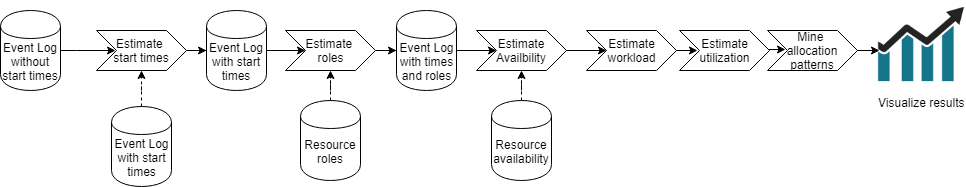
\includegraphics[width=\textwidth]{figures/methodology}
  \caption{High-level methodology overview}
  \label{fig:framework}
\end{figure}



Figure \ref{fig:framework} shows that for each of the three initial steps, it is possible to either provide input data or to estimate the data. In the latter case, the data is estimated and inserted into the event log as a log enhancement part. In the former case, the data is directly inserted as a log enhancement part. The availability estimation is dependent on earlier steps, i.e. roles and event log with start times, and this approach ensures that the analysis is always possible, even without the right data. \todo{Update model such that it is clear that steps can be skipped}

The initial input of the analysis is, just as with other process mining algorithms, an event log. More specially, an event log containing at least the following attributes: \textit{case id}, \textit{event id}, \textit{activity}, \textit{resource} and \textit{event end time}. Furthermore, the following attributes are optional: \textit{event start times}, \textit{other activity lifecycle transitions}, \textit{resource roles} and \textit{resource availability schedules}. Finally, all other case and event attributes, such as \textit{customer type}, \textit{case results} or \textit{organizational hierarchy}, can further enrich the analysis. For the scope of this framework, it is assumed that the event log is complete in the sense that it is represents the actual process execution. 

The next sections each discuss the exact inputs which are necessary for the analysis, the outputs which are generated by the step and which parameters and choices there are in the step. 


\section{Start time estimation} \todo{ToDo}
The first step of the framework is estimating event start times. This step can, of course, be skipped when the event log already contains event start times. 

% What are the inputs? 
% What are the outputs (results) 

% What are the intermediate steps, including choices/parameters. What is chosen and why, and what should be chosen by a domain expert. 

\section{Role Mining}
The next step of the framework is to estimate the roles of the resources including corresponding role hierarchy as defined in RBAC \cite{rbac2, rbac} as explained in section \ref{section:rolemining}. This step requires the activity executions per resource as input data and thus requires only an event log where each event is related to a resource. It is however not uncommon that a domain expert already knows the roles of the corresponding resources and it is also possible to use this information instead of estimating the roles. In this case, it may, furthermore, be interesting to see how the provided roles differ from the estimated roles (i.e., resource role conformance checking). 

Role Mining is, in this framework, defined as a clustering problem, where each cluster corresponds to a role and each data point to a resource. However, clustering itself is not sufficient for mining roles as it does not take into account the role hierarchy and the fact that resources can have multiple roles. The framework does include several heuristics to overcome this issue. 

The role mining outputs, for each resource, one or more roles and the role hierarchy of the event log. Similar to RBAC, employees can have multiple roles, while each role can have multiple related resources. Furthermore, a role can subsume other roles, thus resulting in a hierarchy of roles. Role mining step consists of seven steps. The sections below discuss each sub-step including an overview of all relevant parameters. 

\subsection{Generate input features}
The first step of role mining is to decide on the basis of which information the resources should be grouped into roles. RBAC roles are defined as a set of  permissions, whereas a permission $P$ can defined as pair of granted operations $OPS$ on certain objects $OBS$ \cite{rbac2, rbac}. In the context of role mining, there is only a single relevant permission, namely the right to execute a certain activity. Furthermore, the set of objects can simply be defined as all activities of a process. 

It makes sense to use this information directly as input features. Let $\#_{a}(e)$ be the activity of event $e$. The set of activities of a process can be mined and is defined as $acts(c) = \{\#_{a}(e) | e \in c\}$ and $acts(l) = \bigcup_{c \in l} acts(c)$ for case $c$ and event log $l$, respectively. Similarly, the set of resources can be defined as $res(c) = \{\#_{r}(e) | e \in c\}$ and $res(l) = \bigcup_{c \in l} res(c)$ for case $c$ and event log $l$.  

The actual input features can be defined as the relative frequency of activity executions per resources. Equation \ref{def:inputfeature} formalizes the relative activity frequency for a resource-activity pair, where $\#_{r}(e)$ equal to the related  related resource of event $e$. The relative activity frequency in Equation \ref{def:inputfeature} is defined as the number of times a resource performs an activity normalized by the resource's total activity executions. The normalization ensures that the sum of the relative activity frequencies of a resource is always equal to one. Without the normalization, the scores are dependent on how many events a resource performed in total, which should not influence the role definitions. 

\begin{equation}\label{def:inputfeature}
  \begin{array}{l}
    relative\_activity\_frequency(r,a) =  
    \cfrac{| \{e \in l | \; \#_{a}(e) = a \wedge \#_r(e)=r\}|}
    {| \{e \in l | \; \#_r(e)=r\}|}
  \end{array}
\end{equation}

Additionally, it is recommended to filter the relative activity frequency such that a score is only assigned when resource performed an activity a certain number of times. This prevents that resources which executed only a small amount of events distort the input features, e.g. when a resource only performs activity A, it gets a relative activity frequency of one while this can also be classified as noise. The filtered score is defined in Equation \ref{def:inputfeature_filtered} and only returns a score when the number of activity executions are higher than threshold $t$. The choice of $t$ is dependent on the event log, and can for example be defined as $(|\{e \in l\} \; / \; |res(l)|) \; / \; |acts(l)|)$, which is the activity frequency when a resource randomly performs activities. 


\begin{equation}\label{def:inputfeature_filtered}
  \begin{array}{l}
    rel\_act\_freq\_filtered(r, a, t) = 
    
    \begin{cases}
    	relative\_activity\_frequency(r,a), & \text{for } | \{e \in l | \; \#_r(e)=r\}| > t\\
        0 & \text{otherwise}
    \end{cases}
  \end{array}
\end{equation}

Moreover, the complete input feature is a $R  *  A$ matrix, where $R = res(l)$ and $A = acts(l)$, such that for each resource there is a relative activity frequency for all activities. Furthermore, it is possible to filter all resources which did not perform any tasks or almost any tasks. One can again define a certain threshold and check whether the sum of all activity executions are higher than the threshold. All resources which do not meet the threshold can be removed from the $R  *  A$ matrix.

\subsection{Pick Distance Metric}
The next step is to define a method which is able to check how (dis)similar resources are. These methods are known as distance function. Some well-known examples are euclidean distance, cosine distance and Manhattan distance. There is no distance function which works best on all event logs, thus the distance function should be chosen by a domain expert. 

The definition of these distance functions are shown below in Equation \ref{def:distance_euclidean}, \ref{def:distance_cosine} and \ref{def:distance_manhatten}, where $\mathbf{p}$ and $\mathbf{q}$ are two vectors representing resources, where each element in the vectors correspond with a relative activity frequency: $\mathbf{p}=(p_1,p_2,\dots,p_{|acts(l)|})\text{ and }\mathbf{q}=(q_1,q_2,\dots,q_{|acts(l)|})$.

\begin{equation}\label{def:distance_euclidean}
  \begin{array}{l}
    euclidean\_distance(\mathbf{p},\mathbf{q}) = \sqrt{ \sum_{i=0}^{|acts(l)|}(p_i- q_i)^2}
  \end{array}
\end{equation}


\begin{equation}\label{def:distance_cosine}
  \begin{array}{l}
    cosine\_distance(\mathbf{p},\mathbf{q}) = \frac{ \sum\limits_{i=0}^{|acts(l)|}{p_i  q_i} }{ \sqrt{\sum\limits_{i=0}^{|acts(l)|}{p_i^2}} \sqrt{\sum\limits_{i=0}^{|acts(l)|}{q_i^2}} }
  \end{array}
\end{equation}


\begin{equation}\label{def:distance_manhatten}
  \begin{array}{l}
    manhatten\_distance(\mathbf{p},\mathbf{q}) = \sum_{i=0}^{|acts(l)|} |p_i-q_i|
  \end{array}
\end{equation}

\noindent
The distance functions each work best in certain scenarios. The overview below discusses when the effect of the distance functions and in which situations they generally perform best in the context of role mining. Manhatten distance fits the data best because it evaluates the features completely independent and thus do not assume any relation between the features, contrary to euclidean and cosine distance. 

%However, Manhatten does not perform in all situations best. 

\begin{itemize}
\item \textbf{Euclidean} calculates the shortest distance between two points but is  sensitive to noise. It therefore performs best when there are many resources but not much noise in activities. 
\item \textbf{Cosine} calculates the angle between two vectors but ignores the magnitude of the vector. Therefore, it generally generates less roles and looks more at which relative activity frequencies are positive rather than the difference in scores. It is thus effective in situations where there are many activities and resources and is less sensitive to noise.
\item \textbf{Manhatten} sums the difference between all relative activity scores of resources and therefore is sensitive to small differences in the scores. This results generally in more roles and a more extensive role hierarchy. This distance function is most usable in cases where there are many resources with low number of activities.   
\end{itemize}

\subsection{Additional Preprocessing steps}
It is, furthermore, possible to include other common clustering preprocessing steps such as removal of uncommon activities and feature-wise normalization. This may be valuable in certain situations, but in general both preprocessing steps seem to have a negative effect on the results. The filtering of uncommon activities removes information from the input vectors. The fact that certain resources did not execute certain tasks is also valuable information. 

Furthermore, the feature-wise normalization also seems to impact the output quality in a negative way. Feature-wise normalization ensures that averages and variances within features become equal which has the effect that non-common activities become more important. This effect is clearly shown in Table \ref{table:input} and \ref{table:input_normalized} where Table \ref{table:input_normalized} contains the normalized features of Table \ref{table:input}. In this example, \textit{Activity B} is generally less common in the dataset, but the normalization causes a small difference in relative activity frequency score of \textit{Activity B} is seen as a large change. 

The normalization might be useful for situations where each activity is equally important. However, in most situations there are activities which are more prominent than other activities and thus the normalization might create a distorted view on the dataset. 

\begin{table}
  \parbox{.45\linewidth}{
    \centering
    \begin{tabular}{cccc}
    \hline
    Resource& Activity A & Activity B & ... \\
    \hline
	User\_1 & 0.3 & 0.1 & ... \\
	User\_2 & 0.8 & 0.2 & ... \\
	User\_3 & 0.6 & 0.1 & ... \\
    \hline
    \end{tabular}
    \caption{Example relative activity frequencies input vector}
    \label{table:input}
  }
\hfill
  \parbox{.45\linewidth}{
    \centering
    \begin{tabular}{cccc}
    \hline
    Resource& Activity A & Activity B & ... \\
    \hline
	User\_1 & 0 & 0 & ...\\
	User\_2 & 1 & 1 & ...\\
	User\_3 & 0.5 & 0 & ...\\
    \hline
  \end{tabular}
  \caption{Example input vector normalized with min-max normalization}
  \label{table:input_normalized}
}
\end{table}

Finally, when there are hundreds or even thousands of different activities, or performance is essential, it is also possible to consider a form of dimensionality reduction such as Principle Component Analysis (PCA). In general, dimensionality reduction reduces the time required for clustering but reduces the quality of the clustering. However, when the dataset contains a lot of noise, it may actually yield positive results. When applying dimensionality reduction, it is more challenging to interpret the results, i.e. see why certain resources are clustered together. 

\subsection{Clustering Algorithms}
The next step is to find the best clustering algorithm. There are seven different types of clustering algorithms and the overview below summarises the types and discusses their usefulness for role mining. \todo{sources}

\begin{itemize}
\item \textbf{Centroid-based clustering} aims to optimize the cluster centroid locations by iteratively moving the centroids such that the distance between each cluster and related data point is minimized. The algorithm requires the number of clusters as input which is most of the cases unknown.  
\item \textbf{Fuzzy clustering} is similar to centroid-based clustering but does not limit data points to a single cluster. In practise, this means that a resource can have a relation with multiple clusters, which is also the case with roles. This approach  requires, besides the number of clusters, a 'de-fuzzyfier' which converts the fuzzy relationships to role participation relations. The de-fuzzifier is sensitive to noise and therefore hard to optimize.  
\item \textbf{Agglomerative clustering} initially considers all data points as clusters and merges the two most-similar clustering until there is only a single cluster. The challenge of this approach is to find the best point to stop merging clusters. The advantage of this approach is that it naturally contains a cluster hierarchy which can be used as role hierarchy. However, it does not evaluate all cluster combinations, rather the local best solution which might not be the optimum solution. 
\item \textbf{Graph-based clustering} considers the clustering as a graph optimization problem and tries to find optimal sub-graphs, i.e. clusters, by iteratively cutting the graph in two sub-graphs. This approach also requires the number of clusters as input. Furthermore, this approach does not scale well with the number of clusters and can therefore not be used with large datasets. 
\item \textbf{Density-based clustering} iteratively finds neighbouring data points by checking whether there are any points within a certain range of cluster edges. This approach clusters points based on how similar they are to points in the cluster. This means in practise that not all resources in a clusters should behave as the cluster average, but rather comparable resources are grouped together based on their similarity with the edges of the clusters. The clustering algorithms requires the maximum range parameter which one point can be apart of a cluster (epsilon) and the minimum points per cluster.  
\item \textbf{Distribution-based clustering} This clustering approach does not scale well and can therefore not be used with large datasets. \todo{add description}
\item \textbf{Apriori Rule Mining} approaches to find 'rules' which meet a certain support and confidence threshold. Each rule relates employees to a set of activities. The approach keeps trying to find more complex rules based on the simple rules which meet the threshold, therefore yielding a tree-hierarchy between rules. This approach is, however, very sensitive to noise and generates already thousands of rules for relative small event logs. Furthermore, this approach is also computational expensive and does, therefore, not scale well. 
\end{itemize}

\noindent
The graph-based, distribution-based clustering and apriori rule mining approaches do not scale well with the number of data points and number of clusters and are therefore not usable in practise. Additionally, Fuzzy clustering performs poorly when there is a low amount of noise and therefore is also not usable in practise.

Density-based clustering fits the problem best because it aims to find similar resources based on their distances with their most-similar colleagues and is therefore better in handling slight variations in roles. Centroid-based clustering might be useful when there is low variation between employees, which occurs for example if there are not many activities. Finally, Agglomerative clustering may be useful when there is a lot of variation between clusters. 

Instead of choosing a clustering algorithm beforehand, the most usable algorithms (Density-based, Centroid-based and Agglomerative clustering) can be considered at the same time. The results of each algorithm can be compared and the best can be chosen by a domain expert.  

\subsection{Hyperparameter optimization}
The next step is to optimize the parameters of the chosen algorithms, which includes two important artifices, namely: an evaluation metric and the parameters of the clustering algorithms. When the right evaluation metric is chosen, it is possible to perform a Grid-search approach, i.e. testing each combination of algorithms and possible parameter combination. Other hyper-parameter tuning approaches such as Random Search, Bayesian optimization or Evolutionary optimization can also be used for performance reasons, but this only becomes relevant for very large event logs (e.g. thousands of resources and activities). Gradient-based optimization For performance reasons, the maximum number of iterations for the clustering algorithms can be limited. 

\subsubsection{Evaluation Metric}
Role Mining is defined as an unsupervised clustering problem, and therefore it is not possible to evaluate the results with the absolute truth as this information is unavailable. There are, however, other evaluation metrics for unsupervised clustering which are categorized as internal performance metrics which aim to evaluate goodness of a clustering structure without external information \cite{thalamuthu2006evaluation, dudoit2002prediction}. A well-known example of such a metric is the Silhouette index \cite{rousseeuw1987silhouettes}, which aims to measure how well data points belong in a cluster \cite{rousseeuw1987silhouettes}.

Other internal performance metrics include Davies–-Bouldin index, Dunn index, Calinski-Harabasz, Hubert-Levin (C-index) and Krzanowski-Lai index. Most of these metrics have either a positive or negative trend over the number of clusters, which make them challenging to use for hyperparameter optimization. This is not the case for Silhouette index, Dunn index and Davies-Building index and therefore these metrics are considered in the hyperparamter optimization. \todo{sources}


\subsubsection{Parameters}
Clustering algorithms have different parameters, and therefore the parameter optimization is different for each set of clustering algorithms. DBSCAN has two attributes, namely: the minimum data points in a cluster and the maximum distance between a data point and a cluster edge (epsilon). The former is relative simple as RBAC supports the fact that there is only a single resource related to a role as is discussed in section \ref{section:rolemining}. It therefore does not make sense to choose a higher value. 

However, the epsilon value is more challenging to optimize as it depends on the input features. It is, however, possible to reason about the maximum distance of a dataset, namely: each resource has $|acts(L)|$ number of relative activity frequency scores which range from zero to one. The maximum possible distance in the dataset is thus simply the number of activities. A possible improvement would be to calculate the maximum distance between resources in the event log by taking the maximum value of the distance matrix. It is then possible to try different epsilon values between zero and this maximum and to pick the epsilon with the best performance. 

The centroid-based and agglomerative clustering approaches both only have a single parameter, namely: the amount of clusters (k). It can be optimized is a similar way as the epsilon parameter by checking which k-value performs best. The maximum possible k-value is $|res(l)|$ and the minimum value is two. It is possible to simply evaluate all possible k-values in this interval. However, for datasets with many resources, it is possible to set a maximum to the amount of clusters, e.g.  $|res(l)| / 2$ which only evaluates situations where roles contains, on average, two resources (which is reasonable when considering that RBAC tries to maximize the amount of resources per role \cite{rbac2}).  

\subsection{Prediction}
Based on the output of the hyperparameter optimization, an algorithm with corresponding parameters is chosen. The clustering process is than repeated with a higher number of maximum iterations resulting in a $role(r)$ for each resource $r$. Let $Rs$ be defined as $Rs \;=\; \{role(r) \; | \; r \in res(l)  \}$. 

\subsection{Post-process and decompose roles}
The final step is the post-processing of the clusters into roles. The first step is to place all non-active resources which were removed from the dataset in a new "non-active" cluster. 

The following step is specific to DBSCAN, which places certain resources into an outlier cluster. These resources are not related to each other and therefore the resources should be placed each in their own cluster. 

Next, the clusters should be decomposed into roles by creating a role hierarchy. Each cluster is considered to represent either a single role or a set of roles. In order to find the role hierarchy, the roles are compared with each other. The first step to do so, is to calculate the average relative activity frequency for each role. Next, a single role (source role) is picked and compared to all other roles (target roles). If all activities of a target role, which have a higher average relative activity frequency than threshold $1/|acts(L)|$ (the score which is obtained when randomly performing activities), are also performed by the source role, the target role is considered to be a child-role of the source role. Equation \ref{def:sub_role} formally defines the sub-role relation between role ${r1}$ and role ${r2}$, given threshold $t$ and $r_i$ being defined as the $i^{th}$ average relative activity frequency of role $r$. Equation \ref{def:sub_roles} iterates over all roles ${Rs}$ to find all sub-roles of role ${r1}$.

\begin{equation}\label{def:sub_role}
  \begin{array}{l}
    is\_sub\_role({r1},{r2}, t) = \forall_{i=0}^{|acts(l))|}  \; {r1}_i > t \Rightarrow {r2}_i > t
  \end{array}
\end{equation}

\begin{equation}\label{def:sub_roles}
  \begin{array}{l}
    sub\_roles({r1},{Rs}, t) = \{r \in Rs \; | \;is\_sub\_role({r1}, {r})\}
  \end{array}
\end{equation}

\begin{table}[h]
  \parbox{.45\linewidth}{
    \centering
    \begin{tabular}{cccccc}
    \hline
    Resource& A & B & C & D & Role\\
    \hline
	User\_1 & 0.4 & 0 & 0.4 & 0.2 & 1 \\
	User\_2 & 0.9 & 0.05 & 0.0 & 0.05  & 2  \\
	User\_3 & 0.2 & 0 & 0.4 & 0.4 & 1 \\
    User\_4 & 0.3 & 0.15 & 0.15 & 0.4 & 3 \\
	\hline
    \end{tabular}
    \caption{Example role clustering results}
    \label{table:role_avg}
  }
\hfill
  \parbox{.45\linewidth}{
    \centering
    \begin{tabular}{ccccc}
    \hline
    Role& A & B & C & D\\
    \hline
	1 & 0.3 & 0 & 0.4 & 0.3 \\
	2 & 0.9 & \sout{0.05} & 0 & \sout{0.05}\\
	3 & 0.3 & \sout{0.15} & \sout{0.15} & 0.4\\
    \hline
  \end{tabular}
  \caption{Role averages with filtered scores, threshold: $1/|acts(L)|=0.2$}
  \label{table:role_avg_filtered}
}
\end{table}

Table \ref{table:role_avg} and \ref{table:role_avg_filtered} illustrate this process, where Table \ref{table:role_avg} contains the relative frequency scores for each resource including the predicted role and Table \ref{table:role_avg_filtered} contains the filtered role averages. In this example, role 2 will be classified as sub-role of both role 1 and role 3 because all the roles have a higher average relative activity frequency than role 2 and role 2 does not perform any other tasks than role 1 and 3 which meet the threshold. Furthermore, role 1 also subsumes role 3, as it performs all activities as role 3. The role hierarchy is thus defined as $\{sub\_roles({r1}, t)=\{{r2},{r3}\}, sub\_roles({r2}, t)=\emptyset, sub\_roles({r3}, t)=\{{r2}\}$ for $t = \dfrac{1}{|acts(L)|}=0.2 \}$ as results of Equation \ref{def:sub_roles_hierachy}.

\begin{equation}\label{def:sub_roles_hierachy}
  \begin{array}{l}
    sub\_role\_hierachy(t) = \{sub\_roles(r, t) \; |\; r \in Rs\}
  \end{array}
\end{equation} 

\todo{Add dashboard?}

\section{Availability}
The next step of the framework uses the (estimated) roles and start times to estimate the availability of each resource and each role. It is again possible that the domain expert already has this information and therefore this step might be skipped. In this case, it would be interesting to compare the provided availability with the output of this analysis. The availability analysis has significantly less parameters and choices than role mining.

The availability estimation outputs the times when a resource is generally available in two granularities, namely: the weeks a resource is available and the general work-schedule per weekday. The work-schedule contains for each weekday the half-hour timeslots that a resource is generally available. The reason for the choice of these two granularities is that weeks and workdays are both logical ways to divide a resource's time. The following section discuss how these two availability granularities are calculated.  

\subsection{Available weeks}
The first step of the availability analysis is to check which weeks resources are active. This is important because certain resources may start or stop working on the process during duration of the event log. Furthermore, resources can go on holidays or take time off, which would distort the analysis when is not taken into account. First, the time range of the event log is defined as $weeks(l)=\{ week(\#_{te}(e)) \; | \; e \in l \}$ where $week(\#_{te}(e))$ is the ISO8601 week-number \cite{iso8601} of $\#_{te}(e)$, i.e. the completion time of the event. 

\begin{equation}\label{def:events_per_week}
  \begin{array}{l}
    events\_in\_week(r, week) = \{ e \; | \; e \in l \wedge week(\#_{te}(e)) = week \wedge \#_{r}(e) = r \; \wedge \neg \; \#_{a}(e)\}
  \end{array}
\end{equation}

\begin{equation}\label{def:automated_events}
  \begin{array}{l}
    \#_{a}(e) = \#_{te}(e) - \#_{ts}(e) = 0
  \end{array}
\end{equation}

Next, Equation \ref{def:events_per_week} finds the executed events per week per resource, where $\#_{a}(e)$ is true when the event is classified as an automated event and false otherwise. The definition of automated events can differ between event logs but can be described as system events which are automatically performed by the system or automatically triggered when resources perform certain actions. It is important to filter out the automated events because they are not performed by the resource but rather by the system and therefore do not contain any information regarding the availability of this resource. A method to identify automated events can be found in Equation \ref{def:automated_events}, which simply checks whether the throughput time of an event is equal to zero. 

\begin{equation}\label{def:events_per_week_avg}
  \begin{array}{l}
    avg\_events\_in\_week(r) = avg(w  \in weeks \; | \; weeks_{P^{95}} > events\_in\_week(r, w) > weeks_{P^{5}})
  \end{array}
\end{equation}

\begin{equation}\label{def:active_week}
  \begin{array}{l}
    is\_active\_week(r, week) = \dfrac{avg\_events\_in\_week(r)}{5} < events\_in\_week(r, week)
  \end{array}
\end{equation}

Figure \ref{fig:available_weeks} uses the equations by visualizing the size of the $events\_in\_week$ for all weeks of a single resource where each bar represents a week and the height of the bar represents the number of events executed in this week. Furthermore, the Figure shows a black line which represented the average number of events per week when excluding the top and bottom five percentile of weeks as is defined in Equation \ref{def:events_per_week_avg}. The top and bottom percentiles ($weeks_{P^{95}}$ and $weeks_{P^{5}}$) are removed to prevent outlier weeks from having a large impact on the averages.

Moreover, the bars are coloured red when the weeks do not meet threshold $t$ and coloured green otherwise. The threshold $t$ can again differ between event logs and should be defined by a domain expert, but a method to determine it is to divide the average executed events per week by five as is shown in Equation \ref{def:active_week}. This would imply that if a resource does the same amount of work in a week what it normally does in a single workday (provided that a resource works five workdays a week), it is considered as inactive that week. 

\begin{figure}[h]
	\centering
    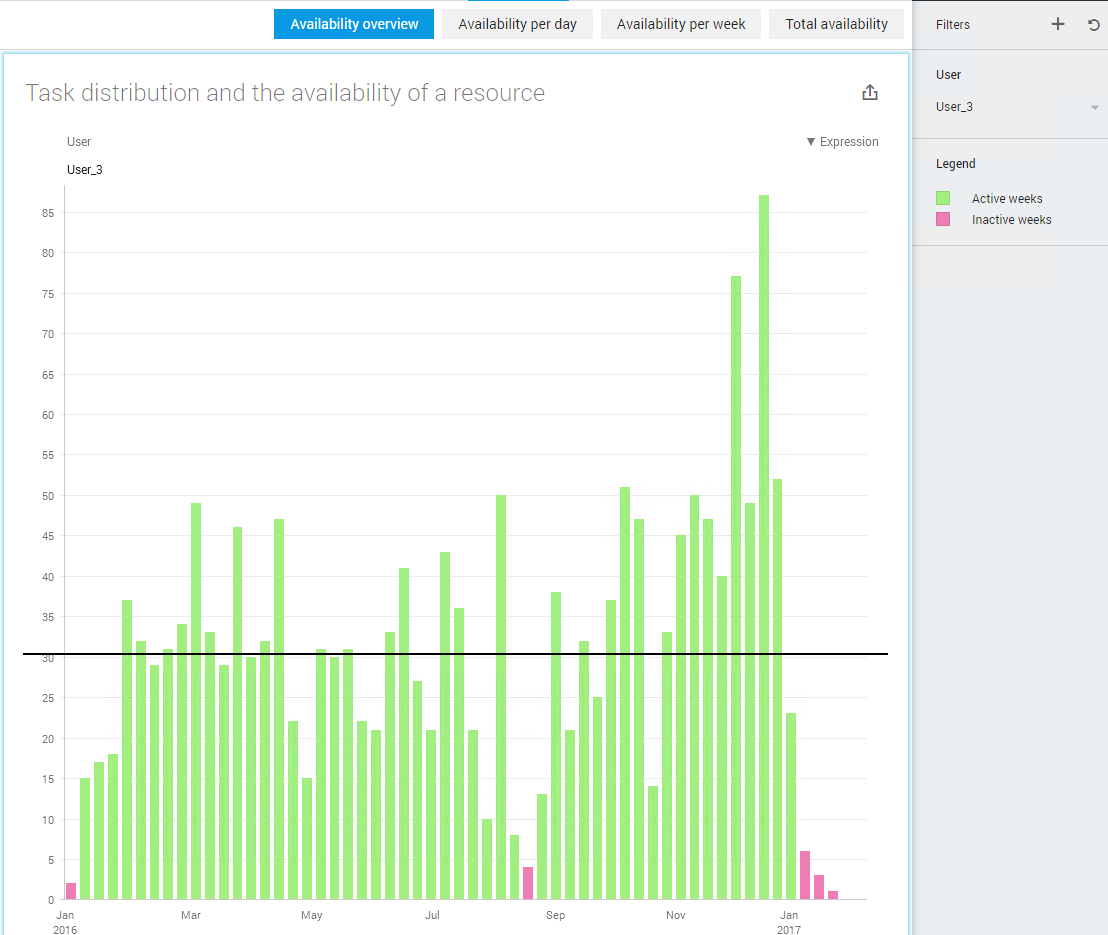
\includegraphics[width=\textwidth]{figures/available_weeks}
    \caption{Events executed per week for resource \textit{User\_5} of the BPIC2017 challenge including the average events per week.}
    \label{fig:available_weeks}
\end{figure}

\subsection{Available timeslots}
This section elaborates on the previous section by finding the availability of resources in preciser time periods of thirty minutes. For each weekday, forty-eight thirty-minutes periods are defined which totals 336 timeslots. Let $ts$ be the set of all timeslots for a week. For each timeslot and for each user the events are counted independent of the weeks. The timeslots are defined per weekday because it is assumed that resources may act differently depending on the weekday. The events per timeslots are only dependent on the available weeks, as only the active weeks are taken into account as is shown in Equation \ref{def:events_per_timeslot}. Similar to the previous section, it is possible to define a threshold for each timeslot to determine when a resource is generally available. 

\begin{equation}\label{def:events_per_timeslot}
  \begin{split}
    events\_in\_timeslot(r, timeslot) = \{ e \; | \; e \in l \wedge is\_active\_week(week(\#_{te}(e))) \; \wedge & \\
    \#_{te}(e) \in timeslot \wedge \#_{r}(e) = r \; \wedge \neg \; \#_{a}(e)\} & 
    \end{split}
\end{equation}


\begin{figure}[h]
	\centering
    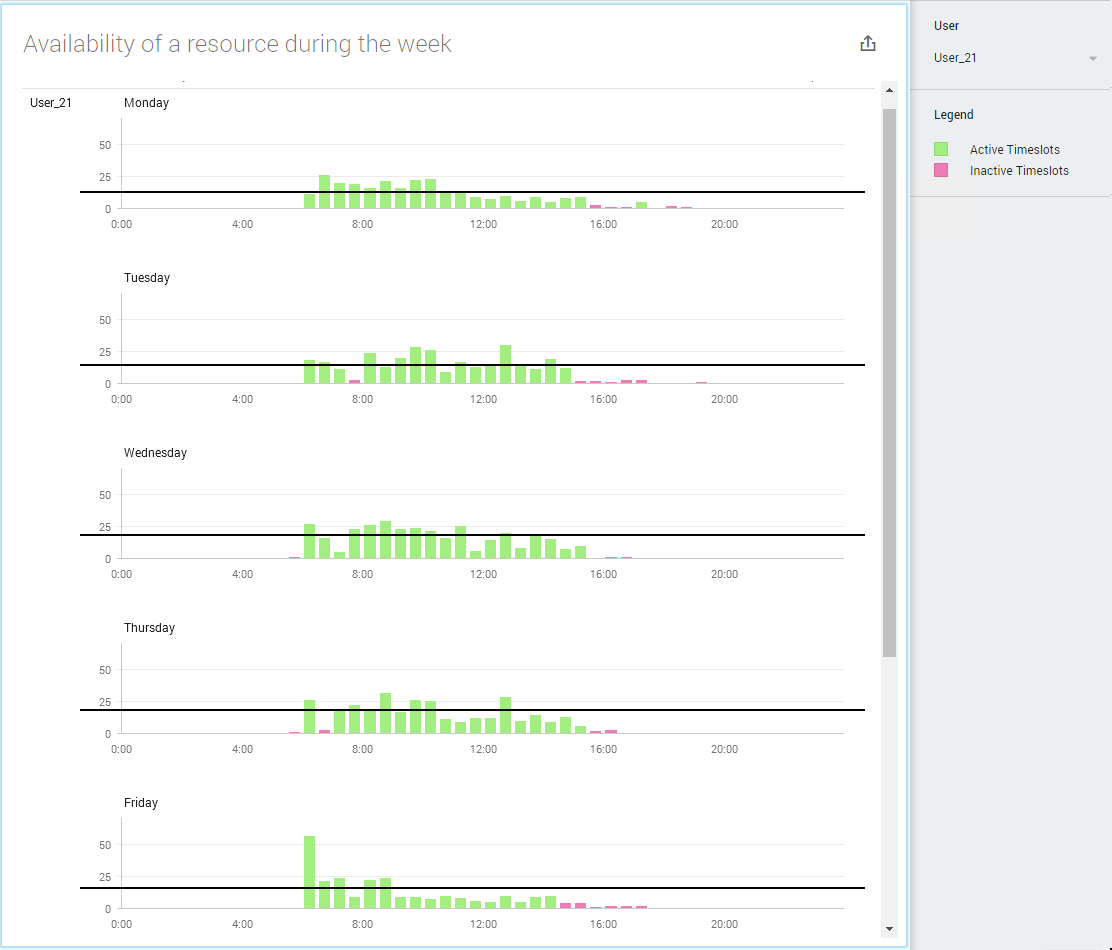
\includegraphics[width=\textwidth]{figures/available_timeslots}
    \caption{Events executed per timeslot for resource \textit{User\_21} of the BPIC2015 challenge including the average events per week.}
    \label{fig:available_timeslots}
\end{figure}

Figure \ref{fig:available_timeslots} illustrates the events per timeslot for resource \textit{User\_21} of the BPIC2017 event log. The Figure shows per weekday the events per timeslot and shows a clear pattern that the resource starts at 6:00 each morning and works until approximately 15:30. However, on Saturday and Sunday, \textit{User\_21} does not seem to work which is rather common in a forty hour work-week. Moreover, the resource seems to leave an hour earlier on Friday. Furthermore, resources may work only part-time and therefore not available on multiple other weekdays. This supports the assumption that resources might have different behaviour on each weekday. 

\begin{equation}\label{def:events_per_timeslot_avg}
  \begin{split}
    avg\_events\_of\_weekday(r, wd) = avg(\{t \in ts \; | \; weekday(t) = wd \; \wedge & \\ 
    ts_{P^{95}} > events\_in\_timeslot(r, t) > ts_{P^{5}} & \})
  \end{split}
\end{equation}

\begin{equation}\label{def:active_timeslot}
  \begin{array}{l}
    is\_active\_timeslot(r, t) = \dfrac{events\_in\_timeslot(r,t)}{5} < avg\_events\_of\_weekday(r, weekday(t))
  \end{array}
\end{equation}

Moreover, the Figure contains green and red colouring which have similar meaning as in Figure \ref{fig:available_weeks}, it indicates whether the timeslots meets a certain threshold. The threshold is defined in Equation \ref{def:active_timeslot} which uses Equation \ref{def:events_per_timeslot_avg}. The latter equation calculates the average events in a certain timeslot and is specific for each weekday $wd$, because it is assumed that resources might have different behaviour dependent on the weekday. Finally, the total available time per resource for the event log can calculated by simply multiplying the active timeslots with the active weeks. 

\section{Workload}
This section elaborates on the availability information by calculating the workload per available timeslot. The workload estimation uses the event start and end times as input and checks at each point of time how 'busy' a resource is. When projecting the workload onto the availability, it is possible to calculate the utilization rate of resources. It is possible to provide the workload and utilization step by manually providing the information. However, it seems rather unlikely that this information is available as it is rather detailed.  

\begin{equation}\label{def:workload_time}
  \begin{array}{l}
    workload(r,t) =  
    | \{e \in l | \; \#_{ts}(e)  \leq t \leq \#_{te}(e) \wedge \#_r(e)=r \; \wedge \neg \; \#_{a}(e)\}| \; 
  \end{array}
\end{equation}

The definition of workload is the amount of events which have started, but have not ended at a certain point of time for a certain resource as can be seen in Equation \ref{def:workload_time}. Again, the automated events are filtered because the resource itself does not perform these events. Moreover, it is possible to calculate the workload in a period of time. It is not possible to simply iterate over all points in time and calculate the workload at all points because time is a continuous value. Furthermore, this would not be an efficient method.   

\begin{figure}[h]
	\centering
    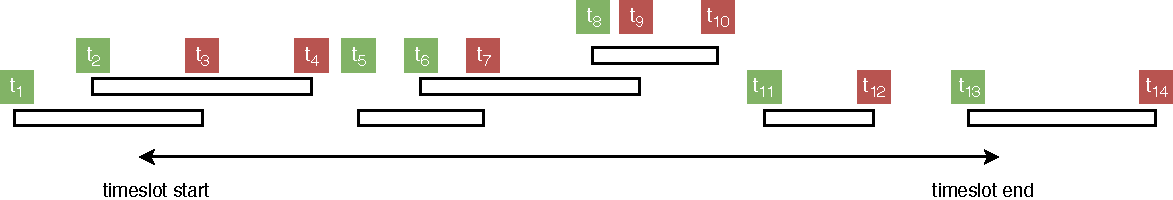
\includegraphics[width=\textwidth]{figures/workload_period}
    \caption{Workload during a time period where green points in time indicate a positive workload delta, and red points in time indicate a negative workload delta}
    \label{fig:workload_period}
\end{figure}

Figure \ref{fig:workload_period} illustrates an alternative method for calculating the workload during a time period. The first step is to filter all events which intersect with the time period, i.e.: $events = \{e \in l | \; \#_{ts}(e) \leq t_e \wedge t_s \leq \#_{te}(e) \; \wedge \#_{r}(e) = r \}$ for resource $r$ and time period $t$ where $t_s$ and $t_e$ denote the start and end times of the period, respectively. Next, it is possible to iterate over the chronological set of start and end times which are denoted in Figure \ref{fig:workload_period} as $t_i$. The workload is static except when an event starts or completes, where the workload is increase or decreased with one, respectively. 

\begin{figure}[h]
	\centering
    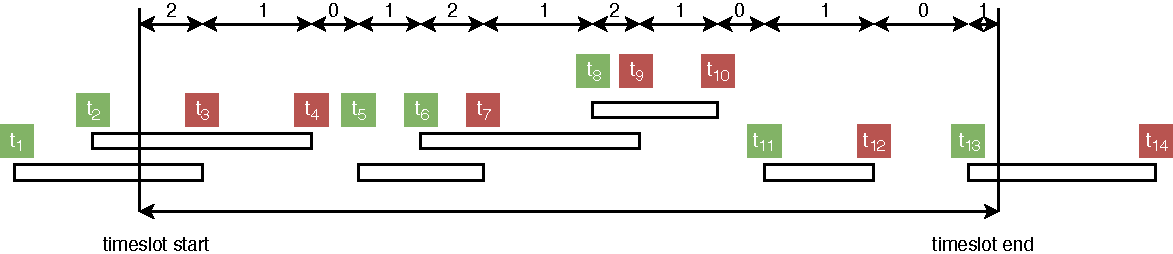
\includegraphics[width=\textwidth]{figures/workload_period_avg}
    \caption{Average workload during a time period where the top numbers indicate the workload for sub-periods of time}
    \label{fig:workload_period_avg}
\end{figure}

This method can be used to calculate the average workload during a time period by slightly extending it. The timeslot start $t_s$ and end $t_e$ should be added to the set of start and end times $t$, but should not decrease nor decrease the workload value. However, the algorithm should only take into account the time between these points for calculating the average workload. The algorithm iterates over this set of times and save the latest point in time which changes the workload as $t_{saved}$. Every time the workload changes, the previous workload value is multiplied with the duration of $seconds(t_{now}) - seconds(t_{saved})$ and the result is saved. The sum of the results divided by the number of seconds per period ($30*60=1800$) equals the average workload during the period. The durations and workload values are illustrated in Figure \ref{fig:workload_period_avg}.

\begin{equation}\label{def:workload_avg}
  \begin{split}
    avg\_workload(r) = avg(\{workload\_per\_period(r,t) | \; (w, t) \in (weeks, ts) \; \wedge  & \\ is\_active\_timeslot(t, w) \wedge is\_active\_week(w)\}) & 
  \end{split}
\end{equation}

By repeating this process for all active periods of a resource, it is possible to calculate the overall average workload per resource as can be seen in \ref{def:workload_avg}. This Equation does, similar to previous equations, only take into account the active weeks and active timeslots.


\section{Utilization}
  This section continues on the availability and workload by calculating the utilization rate. The utilization rate is defined as the sum of idle time during active time divided by the total available time. Figure \ref{fig:utilization_rate} illustrates this by highlighting the idle-periods in blue (the points in time where the workload is zero). The utilization rate can then be calculated by summing the idle durations and dividing it by the period length. When comparing this to the approach of calculating the workload, it would mean that $t_{saved}$ is only updated when the workload goes to zero (e.g. $t_4,t_{10}, t_{12}$) and the result is saved only when the workload goes to one from zero (e.g. $t_5,t_{11},t_{13}$). 


This will result in the utilization rate which is defined from zero to one where zero indicates that the resource is on all times working  and one indicates the the resource is not working during the period. 

\begin{figure}[h]
	\centering
    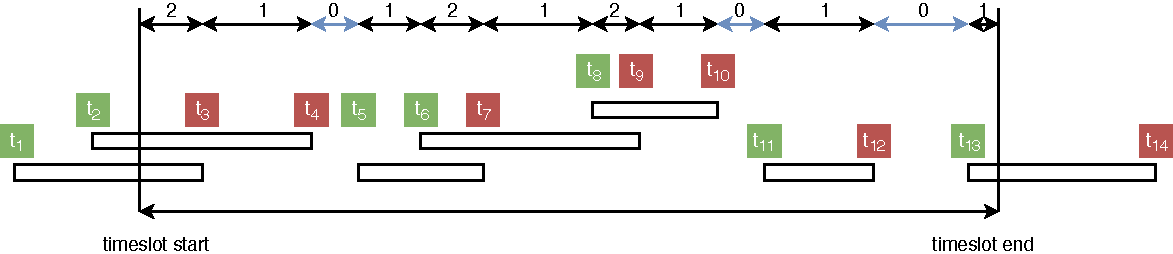
\includegraphics[width=\textwidth]{figures/utilization_rate}
    \caption{Utilization rate during a time period where the top numbers indicate the workload for sub-periods of time}
    \label{fig:utilization_rate}
\end{figure}

\todo{add visualizations of utilization}

\section{Work-allocation patterns}
Finally, all this information can be used to mine resource allocation patterns. The exact input data depends on which resource-allocation patterns should be mined. 

\todo{Implement and report}




